%%%%%%%%%%%%%%%%%%%%%%%%%%%%%%%%%%%%%%%%%%%%%%%%%%%%%%%%%%%%%%%%%%%%%%%%%%%%%%%%
% \documentclass[12pt,papel,twoside]{ibtesis}
%\documentclass[12pt,screen,twoside,pagebackref]{ibtesis}
 \documentclass[12pt,papel,singlespace,oneside]{ibtesis}
% \documentclass[12pt,papel,preprint,singlespace,oneside]{ibtesis}
%%%%%%%%%%%%%%%%%%%%% Paquetes extra %%%%%%%%%%%%%%%%%%%%%%%%%%%%%%%%%%%%%%%%%%%
% Por conveniencia: aqu\'{\i} puede cargar todos los paquetes y definir los comandos 
% que necesite
\usepackage{ibextra}
\usepackage{subfig} %para poner varias imagenes en una sola figura
\usepackage{url} %para citar páginas web
\usepackage{notoccite}
\usepackage{verbatim}
%\usepackage{graphicx}
%\nofiles
%%%%%%%%%%%%%%%%%%%%%%%%%%%%%%%%%%%%%%%%%%%%%%%%%%%%%%%%%%%%%%%%%%%%%%%%%%%%%%%%
%%%%%%%%%%%%%%%%%%%%% Informacion sobre la tesis %%%%%%%%%%%%%%%%%%%%%%%%%%%%%%%
\title{Desarrollo de Texturas: Integraci\'on de la Microestructura mediante Experimentos y Simulaciones}
\author{Mg. Emanuel Alejandro Benatti}
\director{Dr. Raúl Eduardo Bolmaro}
\carrera{Tesis Doctorado en F\'{\i}sica}
\grado{Doctorando}
\laboratorio{Física y Micromecánica de materiales heterogéneos \\ Instituto de Física Rosario}
%\palabrasclave{DETECTOR, SUPERCONDUCTOR, MgB$_{2}$, NEUTRÓN}
%\keywords{detector, superconductor, MgB$_{2}$, neutron}
% Si queremos poner la fecha manualmente:
% \date{Diciembre de 2099}

%%%%%%%%%%%%%%%%%%%%%%%%%%%%%%%%%%%%%%%%%%%%%%%%%%%%%%%%%%%%%%%%%%%%%%%%%%%%%%%%
%\titlepagefalse % Si no quiere compilar la portada descomente esta linea
%\includeonly{apendices} % Compilar s\'{o}lo estos archivos 
%\graphicspath{{figs/}} % Lugar donde encontrar las figuras generales (se puede poner uno en cada cap{\'{\i}}tulo)
%%%%%%%%%%%%%%%%%%%%%%%%%%%%%%%%%%%%%%%%%%%%%%%%%%%%%%%%%%%%%%%%%%%%%%%%%%%%%%%%


\begin{document}

% Dentro del environment 'preliminary' va:
% la dedicatoria, resumen, abstract, indices

\begin{preliminary}

% Escriba su dedicatoria
\dedicatoria{
A mi familia\\
A mis amigos\\
y a todos los que se lo merecen \\
por merecerlo. \\
}

%%% \'{I}ndices %%%%
%\begin{abreviaturas}
%    \printnomenclature
%\end{abreviaturas}

\tableofcontents                %\'{I}ndice

\listoffigures                  %Figuras

%\listoftables                   %Tablas

\listofabbr						%Símbolos y abreviaturas


\begin{resumen}%
  En este trabajo se estudia la viabilidad de utilizar films del supuerconductor MgB$_2$, que tiene una temperatura crítica alrededor de 39\,K, para construir un detector de neutrones térmicos y fríos. El objetivo es aprovechar el calor generado por la reacción $^{10}$B$(n,\alpha)^6$Li que tiene una sección eficaz de 3800\,barns para neutrones térmicos y libera una energía de aproximadamente 2.3\,MeV. El calor producido por la reacción produce una supresión momentánea de la superconductividad, lo que produce una señal que permite registrar la captura de un neutrón. Se realizaron simulaciones de las trayectorias de los productos de la reacción en el MgB$_2$ para estimar las dimensiones del detector que permitan maximizar su señal, sensibilidad y eficiencia, y que minimicen el tiempo de respuesta, al tiempo que se estimó que la energía de la reacción se deposita en un volumen de unos pocos micrómetros cúbicos. Cálculos y simulaciones hechas con el software comercial de elementos finitos COMSOL MULTIPHYSICS llevaron a la conclusión de que para poder detectar eficientemente neutrones con el MgB$_2$, resulta necesario construir un cable que tenga un ancho no mayor a un micrón y un espesor no mucho mayor a los 200\,nm. Dimensiones mayores incrementan la probabilidad de captura de un neutrón pero reducen drásticamente la señal y la sensibilidad del detector, además de que dificultan el control de la temperatura del mismo.

Fueron realizadas simulaciones en las que se acopló la física del comportamiento térmico y eléctrico del detector, y se observó que si el mismo es operado con corrientes lo suficientemente bajas, la señal y el tiempo de respuesta del detector no se modifican, y que tiene un tiempo de respuesta de algunos nanosegundos cuando el espesor del cable es de 200\,nm. También se llevaron a cabo simulaciones intentando regular la temperatura del detector simplemente variando la tensión aplicada al mismo, pero el resultado fue que eso no es posible desde el punto de vista práctico, ya que para regular la temperatura del detector en el rango de interés, es preciso aplicar tensiones que llevan a que circulen corrientes enormes por el cable de MgB$_2$. La conclusión extraída de este cálculo fue que el detector va a requerir un mecanismo adicional para controlar su temperatura. También se concluyó que por razones de estabilidad en el control de la misma, es conveniente operar al detector a tensión constante, en vez de hacerlo a corriente constante.

En conjunto con el trabajo de las simulaciones se intentó crecer films de MgB$_2$ por medio de dos técnicas diferentes, una utilizando un método ex-situ que requrió temperaturas del orden de los 700\,$^{\circ}$C, y otra consistente en un método in-situ que requería temperaturas iban de los de 500\,$^{\circ}$C hasta temperatura ambiente.

La primera técnica de crecimiento consistió en depositar films de B por evaporación para luego recocer los mismos junto con pastillas de MgB$_2$ bulk en ampollas de cuarzo. Se lograron fabricar films de un espesor de algunos cientos de nanómetros, cuyas curvas de magnetización, medidas en un magnetómetro SQUID, presentaron irreversibilidades en un ciclo \textit{Zero Field Cooling - Field Cooling} compatibles con la formación de una fase superconductora. Sin embargo, siguiendo este método no se pudo conseguir fabricar films con una transición superconductora lo suficientemente estrecha como para poder fabricar el detector, lo que probablemente se debió a que el sustrato reaccionaba con el film debido a las elevadas temperaturas del recocido.

La segunda técnica de crecimiento de films de MgB$_2$ explorada en este trabajo fue la de crecimiento directo de films por sputtering, a partir de un blanco de MgB$_2$ obtenido comercialmente. Se realizaron estudios de difracción de rayos X que no mostraron la formación de la fase MgB$_2$. Un estudio de la composición de los films crecidos fue realizado utlizando espectroscopía de rayos X caracterísiticos (EDX) y retrodispersión de Rutherford (RBS). Ambos estudios mostraron que los films crecidos tienen un exceso de B, lo que probablemente sea la causa de que no sean superconductores, tal como mostraron las mediciones de magnetización realizadas sobre las muestras. Se decidió intentar recocer los films crecidos con pastillas de Mg, en busca de mejorar la proporcion B/Mg de los films utilizando una temperatura de recocido más baja que la empleada con los films crecidos por evaporación. El recocido logró una mejora en las propiedades de transporte de las muestras, ya que pasaron de ser aislantes a ser semiconductoras, pero no se pudo observar la formación de fases superconductoras, ni en mediciones de magnetización, ni en mediciones de transporte, lo que consituye un indicio de que los films no lograron incorporar la cantidad suficiente de Mg como para volverse superconductores. Esto último se deba probablemente a que la temperatura de recocido no fue lo suficientemente alta como para permitir la difusión de la cantidad necesaria de Mg a través del film.
\end{resumen}

\begin{abstract}%
	In this paper we study the feasibility of using films of the superconductor MgB$_2$ with a critical temperature of 39\,K, to build a cold neutron and thermal neutron detector. The aim is to use the heat generated by the reaction $^{10}$B$(n,\alpha)^6$Li which has a cross section of 3800\,barns for thermal neutrons and releases an energy of approximately 2.3\,MeV. The heat produced by the reaction causes a partial destruction of superconductivity. One then notices the appearance of a single neutron by the electric resistance variation of the MgB2 thin film. Simulations of the trajectories of the reaction products in the MgB$_2$ were performed for estimating the optimal detector dimensions. Calculations and simulations with the commercial software COMSOL Multiphysics led to the conclusion that in order to efficiently detect neutrons with MgB$_2$, is necessary to build a cable that has a width no greater than one micron and a thickness not much greater than 200\,nm. Larger dimensions increase the probability of neutron capture but drastically reduces the produced signal and the detector sensitivity, plus it difficult the temperature control of the device.

	Simulations were also conducted coupling the physics of the thermal and electrical behavior of the detector, and it was found that if it is operated with a small bias-current, the detector's signal and response time are not changed. Calculations showed that the detector has a response time of few nanoseconds for a wire 200\,nm thick. Simulations were carried out trying to regulate the temperature of the detector by varying the bias tension, but it was found that this is not a viable option from a practical standpoint, as to regulate the temperature of the detector in the range of interest, it is necesary to apply voltages that lead to large currents circulating through the detector. This implied that the construction of the detector will require an additional mechanism to control its temperature. It was also found that for reasons of stability in temperature control, it is desirable to operate the detector voltage-biased instead of current-biased.

	In addition with the simulations, growth of MgB$_2$ films was attempted by two different means, one using an ex-situ method requiring temperatures around 700\,$^{\circ}$C, and an in-situ method requiring temperatures of 500\,$^{\circ}$C down to room temperature.

	The first technique consisted on growing of boron films by evaporation and a post-annealing process with a bulk MgB$_2$ sample in a quartz tube. We managed to make 200\,nm thick films, and perform magnetization measurements in a SQUID magnetoteter. Irreversibilities shown in a Zero Field Coolig - Field Coolig magnetization measurement were compatible with the formation of a superconducting phase. However, it wasn't possible to obtain films with a sharp superconducting transition, as it's needed to build the detector. This is probably the result of a chemical reaction between substrate and the film due to the high annealing temperatures.

  The second technique explored in this work was the direct growth of MgB$_2$ films by sputtering. To this end a commercial MgB$_2$ target was used. Studies performed by X-ray diffraction did not show the formation of the MgB$_2$ crystalline phase. We also studied the composition of the films by electron dispersive X-ray analisys (EDX) and Rutherford backscattering (RBS). Both studies showed that films are grown with an excess of B, which is probably the reason why they are not superconducting, as was observed by magnetization measurements. Films were annealed with Mg pellets, seeking to increase the amount of Mg in the films, using lower annealing temperatures than those used with the films grown by evaporation. Samples showed an improvement in their transport properties after the annealing, as they went from being insulating to semiconductonducting. However no formation of a superconducting phase was observed, neither in magnetization measurements or in electrical resistance measurements. This is probably due to the low annealing temperature, which did not allow the diffusion of the required amount of Mg through the film.
\end{abstract}

%%% Local Variables: 
%%% mode: latex
%%% TeX-master: "template"
%%% End: 

\end{preliminary}


% Podemos usar cualquiera de los dos comandos: \input o \include para incluir el texto
\chapter{Introducci\'on}
\graphicspath{{./figs/01_intro/}}
\chapterquote{La destrucción es obra de una tarde. La creación es obra de una vida.}{Kamahl, acólito druida}
\section{Motivación}\label{S:motivacion}

\section{Difracción de Rayos X}\label{S:DRX}
Los rayos X son una herramienta de vital importancia para el estudio de los materiales cristalinos. 
En la difracción de Rayos X (DRX), un haz monocromático de de rayos X de longitud de onda $\lambda$ incide sobre una dada muestra (Fig. \ref{fig:Bragg}). 
Si el cristal es infinito y está libre de cualquier tipo de distorsiones, para una dada familia de planos ${hkl}$, habrá interferencia constructiva para los haces salientes que cumplan con la condición de Bragg[ref]:

Esto esta medio medio, hay que hablar de que los cristales estan en arreglos periodicos de atomos

\begin{equation}
  2 \ d_{hkl} \ \sin(\theta_{B}) \ = \ n \ \lambda
  \label{eq:Bragg}
\end{equation}
\noindent
siendo $d_{hkl}$ la distancia interplanar de la familia de planos {hkl}, 2$\theta_{B}$ el ángulo formado entre el haz incidente y el haz reflejado y $n$ el número de orden de difracción. 

Hay que pensar en el planteo mas riguroso, usando los vectores K, porque lo voy a necesitar para explicar williamson hall

\nomenclature{$\lambda$}{Longitud de onda}
\nomenclature{$d_{hkl}$}{Distacia interplanar para la familia de planos $hkl$}

\begin{figure}[htb!]
  \centering
  \includegraphics[width=\imsize]{BraggLaw}
  \caption{Ley de Bragg}
  \label{fig:Bragg}
\end{figure}

Una consecuencia de la ley expresada en la Ec. \ref{eq:Bragg} es que para un cierto haz incidente habrá reflexiones cuyas distribución de intensidades serán funciones deltas de Dirac[ref], con intensidad infinita para el ángulo $\theta_{B}$ e intensidad nula para los ángulos $\theta$ que no cumplan con la condición de Bragg. Como resultado, los "picos" de difracción tendrán además un ancho nulo. 
Si, como ocurre en la práctica, el número de planos que contribuyen a la reflexión es finito, la distribución angular de intensidades tendrán un ancho y altura finitos, y lo mismo ocurrirá si la red de átomos tiene distorsiones, es decir, si los átomos no se encuentran en un arreglo perfectamente periódico. 
En un experimento de DRX real aparecerán además otras contribuciones que ensancharán los picos de difracción. 
Por un lado el haz incidente no será puntual ni estará constituido por haces completamente paralelos, sino que tendrá de un tamaño finito y estará comprendido entre haces que tendrán cierta divergencia angular. 
Además, el haz no será completamente monocromático, sino que estará inegrado por rayos X con longitudes de onda en un intervalo $(\lambda \ \pm \ \Delta \lambda)$. 
Todos estos factores cotribuirán a que haya haces difractados en las vecindades de $\theta_{B}$, aumentando el ancho de los picos de difracción.



Hay que hablar de los principios de medicion, rayos X de laboratorio y de sincrotron
Estudio de ancho de pico, Langford, Williamson Hall, Warren Averbach y CMWP

\section{Difracción de electrones retro difundidos}\label{S:EBSD}
Cómo se mide y cómo se pueden relacionar las magnitudes de EBSD con las de RX
Que permite y que no permite ver en comparacion con RX

¿Hablo de TEM?
 
\section{Textura cristalográfica}\label{S:Text}
Definicion de textura, relacion con los procesos de deformacion y la microestructura.
ODF: definicion y obtencion a partir de RX y EBSD. Diferencias de los dos métodos.

\subsection{FDO y FDO generalizada}\label{SS:ODF}
Relacion entre la ODF y la ODF generalizada. Relacion de FWHM y energía de deformacion.

\section{Revisión bibliográfica y estado del arte}\label{S:RB}

\section{Organización de la tesis}\label{S:Org}

\chapter{Materiales y métodos}\label{C:Materiales}
\graphicspath{{./figs/02_Mat/}}
\section{Experimentos de difracción de rayos X}\label{S:MatXRD}
Buena parte del trabajo de esta tesis se centró alrededor de los experimentos de difracción de rayos X.
En particular, la mediciones se hicieron empleando la geometría de transmisión, también llamada de Debye-Scherrer, utilizando radiación sincrotrón.
La facilidad empleada fue PETRA III, cuya fotografía puede verse en la Fig. \label{fig:desy}, y está ubicada en el complejo DESY, en la ciudad de Hamburgo, Alemania\cite{desy}.

\begin{figure}[!htb]
  \centering
  \includegraphics[width=\textwidth]{desy}
  \caption{Fotografías del exterior e interior de la facilidad PETRA III, en DESY. Imágenes obtenidas de \cite{desy}.}
  \label{fig:desy}
\end{figure}

En los experimentos de transmisión realizados, un haz de rayos X con $\lambda \ \approx \ 0.0142$\,nm incide sobre una dada muestra, como se puede apreciar en la imagen de la Fig. \ref{fig:transmision}. 
Como resultado de la interacción elástica entre el haz incidente y el material, diferentes haces con la misma energía que el incidente, son dispersados por diferentes familias de planos en ángulos que están dados por la Ley de Bragg \ref{eq:Bragg}.
Para una dada familia de planos $\{hkl\}$ todos los haces difractados están comprendidos en un cono, que al interceptar el detector forman un círculo, denominado anillo de Debye, y la intensidad del haz difractado a lo largo de largo del anillo de Debye está determinada por la cantidad de planos cristalinos en condición de difracción para esa dada orientación de la muestra.

En la configuración que se muestra en la Fig. \ref{fig:transmision} la muestra se colocó en un portamuestra que permitía la alineación con el haz y el detector, y daba a la muestra la libertad de girar alrededor de un eje vertical que pasaba por su centro.
La muestra rotaba gracias a un motor paso a paso y que permitía rotar con una precisión de 5\,$^{\circ}$.
Para obtener una caracterización completa de la textura de la muestra, fue necesario rotar la misma un rango de 180\,$^{\circ}$, lo que sumado a la resolución en la rotación significa que por cada muestra se obtuvieron 37 anillos de Debye.

\begin{figure}[!htb]
  \centering
  \includegraphics[width=\textwidth]{process}
  \caption{Esquema básico del proceso de medición y análisis de datos. Las mediciones se realizaron empleando una geometría de transmisión, para diferentes rotaciones $\omega$ de la muestra. Por cada posición de la muestra se registraron una serie de anillos de Debye, a partir de los cuales se extrajeron porciones radiales con los que se construyeron los difractogramas que luego fueron procesados siguiendo diferentes modelos microestructurales. A partir de estos resultados, y realizando la conversión adecuada de las coordenadas de laboratorio a las coordenadas del sistema de referencia del cristal, se construyeron figuras de polos y figuras de polos generalizadas.}
  \label{fig:transmision}
\end{figure}

El haz que incidente tiene un tamaño de 100\,$\mu$m x 100\,$\mu$m, lo que permite obener una gran resolución sobre la microestructura del material.
Las muestras empleadas tenían forma de varillas con su eje colocado verticalmente, es decir, paralelas al eje de giro.
El ancho de las varillas era de entre 2\,mm y 5\,mm, y se tuvo especial cuidado durante la alineación de que el haz esté completamente adentro de la muestra en todo el rango de rotación de la muestra.
Se utilizó un detector de estado sólido Mar345 de forma cuadrada, con una grilla de 3450\,pixels x 3450\,pixels, de 100\,$\mu$m x 100\,$\mu$m cada uno.
El detector se colocó 1081\,mm detrás de la muestra, y los tiempos de detección se modificaron de acuerdo a la intensidad de salida del haz y la absorción de la muestra, de modo de que las intensidades máximas siempre estén cerca del número máximo de cuentas medibles por el detector.

De cada medición se extrajeron 37 imágenes, cada una de las cuales contaba con conjuntos de 5 a 7 anillos de Debye, dependiendo de la muestra.
De cada imagen se extrajeron porciones radiales de ancho angular de 5\,$^{\circ}$ a partir de las cuales se construyeron 72 difractogramas.
El conjunto de 72 x 37 = 2664 difractogramas fue analizado utilizando diferentes modelos microestructurales, pero hubo dos modelos sobre los que se hizo especial foco: el CMWP (Sec. \ref{SS:CMWP}) y el de Langford (Sec. \ref{SS:02Langford}), y de cada modelo empleado se extrajo diferente información sobre la microestructura.

Cada pico de cada difractograma quedaba identificado por su ánglulo de Bragg $\theta_B$, su coordenada angular $\gamma$ en el anillo de Debye y la rotación de la muestra $\omega$ cuando se realizó la medición, por lo que la información microestructural era susceptible de ser graficada empleando figuras de polos, del misma manera que se grafican las figuras de polos.
Para construir figuras de polos a partir de las mediciones realizadas es preciso transformar las coordenadas de los picos en el sistema de laboratorio $(\omega, \gamma, \theta_B)$ al sistema de referencia del cristal $(\alpha, \beta)$, para lo cual se empleó la matriz de rotación ya calculada por Bunge y Klein\cite{Bunge1996}.
La misma expresión fue empleada para generar las figuras de polos generalizadas.

\subsection{Contribuciones instrumentales al ancho de pico}\label{SS:inst}
Para poder realizar un análisis microestructural preciso a partir de mediciones de ancho de pico, es necesario dar cuenta del ancho instrumental del equipo empleado.
Se define como ancho instrumental al ensanchamiento que se observa alrededor de los picos de Bragg y que es independiente de la microestructura de la muestra estudiada.
Para medir el ancho instrumental se emplean patrones de laboratorio, es decir, muestras que poseen una geometría similar a la de las muestras a estudiar y que no poseen ensanchamiento (o poseen un ensanchamiento muy pequeño) debido a factores microestructurales, como ser tensiones internas y tamaño de grano.
También es preciso que los patrones instrumentales no posean ningún tipo de textura.
Para las mediciones de este trabajo se utilizó un polvo de LaB$_6$ como patrón instrumental.

\begin{figure}[!htb]
  \centering
  \includegraphics[width=\textwidth]{IF75R_FWHM_Raw_Points_NoSym}
  \caption{.}
  \label{fig:IF75NoSym}
\end{figure}


\begin{figure}[!htb]
  \centering
  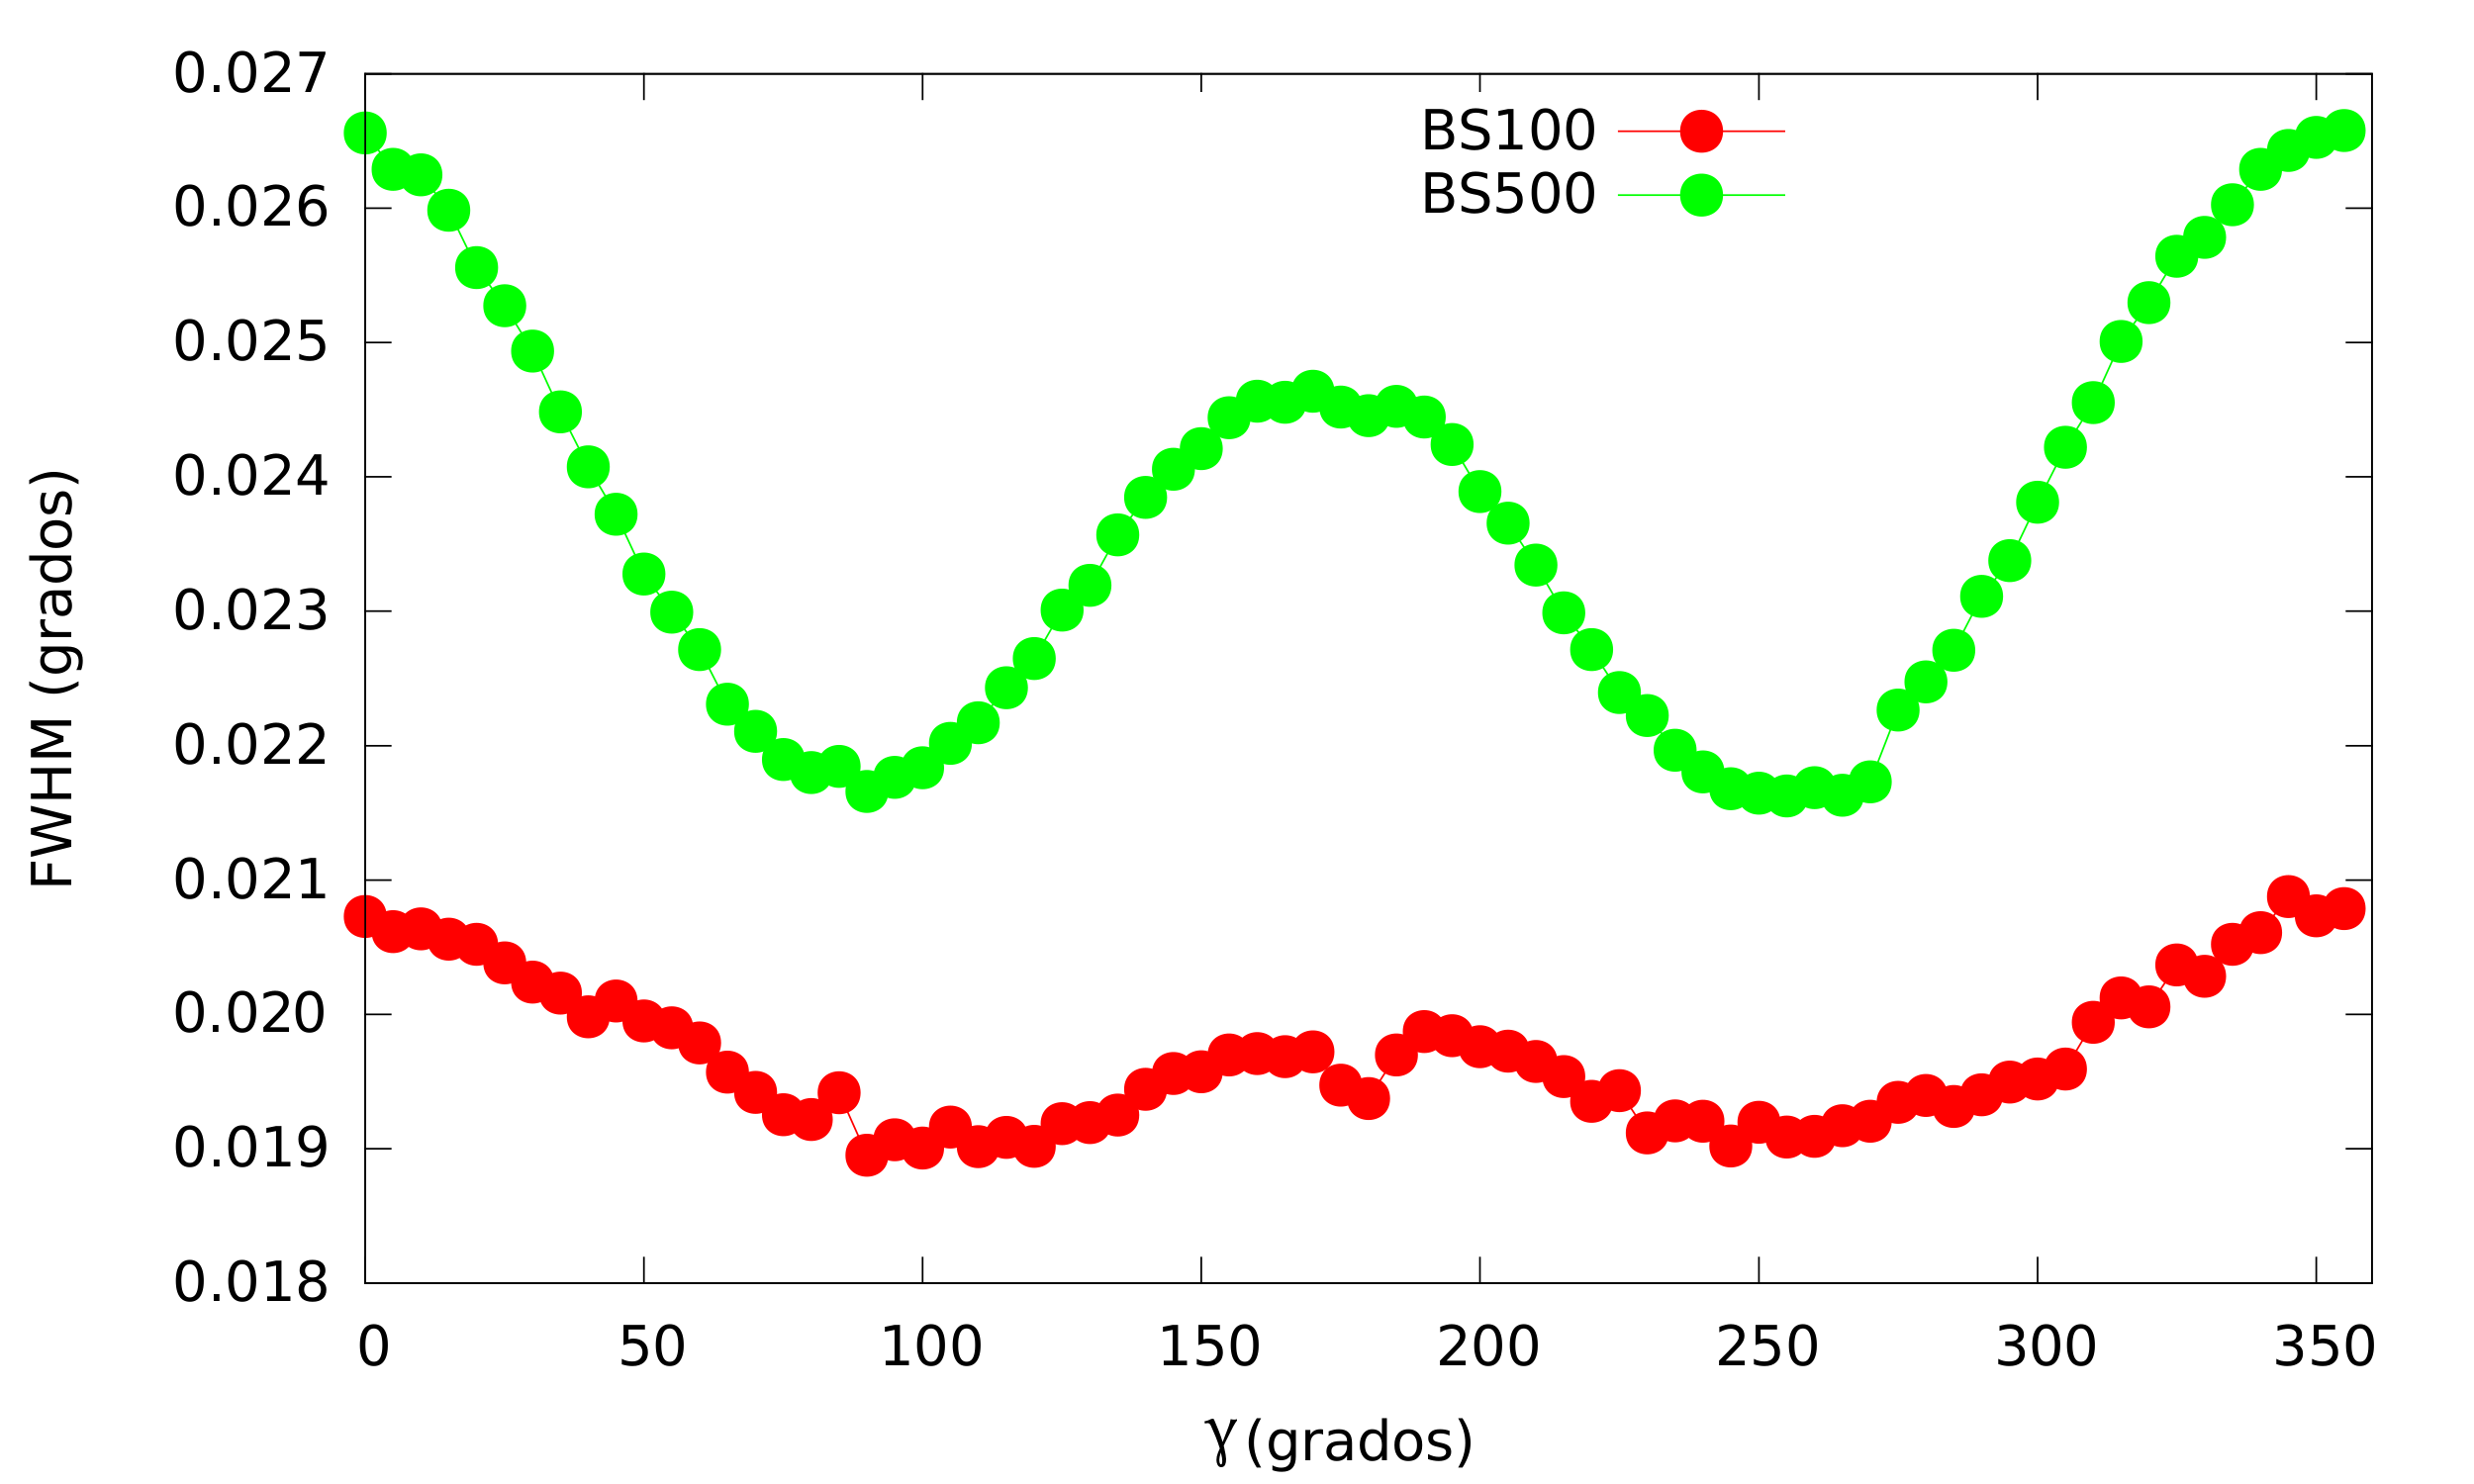
\includegraphics[width=0.8\textwidth]{LaB6_1mm_FWHMvsGammavsBS}
  \caption{Variacion del ancho instrumental como función del ángulo a lo largo del anillo de Debye.}
  \label{fig:LaB6vsGamma}
\end{figure}

\begin{figure}[!htb]
  \centering
  \includegraphics[width=0.8\textwidth]{IF75R_FWHM_Raw_Points_Sym}
  \caption{.}
  \label{fig:IF75Sym}
\end{figure}

\newpage
\subsection{Postprocesamiento de los datos}\label{SS:MatPost}
Para obtener los difractogramas necesarios tanto para medir la textura como para realizar los estudios de ancho de pico, es preciso convertir las imágenes obtenidas de los detectores de estado sólido a archivos de texto con información numérica que pueda ser procesada por programas de computadora.
Las imágenes obtenidas por el detector Mar345 fueron procesadas con el programa FIT2D\cite{FIT2D}, que permitió obtener porciones radiales con $\Delta \gamma \ = \ 5\,^{\circ}$ de ancho para cada conjunto de anillos, permitiendo obtener un difractograma para cada porción radial en la imagen registrada.
Como cada anillo barre un ángulo de 360\,$^{\circ}$, para cada ángulo $\omega$ que representa la rotación de la muestra se obtuvieron 72 difractogramas, cada uno de los cuales tenía asociada una coordenada $\gamma$, que marcaba su posición angular en la imagen extraída del programa FIT2D (Fig. \ref{fig:fit2d}).

\begin{figure}[!htb] 
  \centering
  \includegraphics[width=0.5\textwidth]{Fit2D_2}
  \caption{Para convertir las imágenes grabadas en cada experimento de difracción se empleó el programa FIT2D, que permitió dividir a cada conjunto de anillos de Debye en 72 porciones de 5\,$^{\circ}$ cada una. El programa luego extraía la intensidad de promedio grabada dentro de cada porción y con esa información construía difractogramas que fueron luego empleado para realizar los ajustes.}
  \label{fig:fit2d}
\end{figure}

Una vez obtenidos los 2664 difractogramas, los mismos fueron ajustados con un software de elaboración propia, tanto para aplicar el método de Langford como el CMWP.

Ambos softwares toman como dato de entrada todos los difractogramas obtenidos con FIT2D, además de otros archivos que deben ser escritos por el usuario, y que se encuentran ejemplificados en el apéndice \ref{CA:input}.

En el caso del programa que realiza el análisis de Langford se precisan tres archivos además de los datos extraídos de FIT2D.
El primero se denomina \textit{data\_info\_1.ini} y contiene la información que indica dónde se guardarán los resultados y dónde se encuentran los archivos de entrada, así como su cantidad y los datos necesarios para realizar la conversión angular.
También la resolución en píxeles del detector y la distancia entre el detector y la muestra, datos necesarios para convertir las distancias sobre el detector a la variable 2$\theta$.
La opción \textit{Treshold} es un dato numérico que se emplea para determinar cuál es la intensidad mínima por encima del ruido de fondo que debe tener un pico para ser ajustado por el método de mínimo cuadrados. 
Como ajustar picos de baja intensidad puede llevar a alargar el tiempo que lleva procesar los datos, además de dar resultados poco confiables, no se recomienda colocar 0 como valor de umbral, mientras que un valor de 5 ha dado buenos resultados para las mediciones realizadas en esta tesis, como se puede ver en la Fig. \ref{fig:MinIntensity}

\begin{figure}[!htb]
  \centering
  \includegraphics[width=0.8\textwidth]{Pico_minimo}
  \caption{La relación señal ruido mínima que permite distinguir y ajustar apropiadamente un pico del difractograma. El pico que se muestra tiene una intensidad integrada neta de 5 y como puede verse es ajustado razonablemente por una función pseudo-Voigt. Si el pico es más pequeño el error del ajuste se vuelve muy grande e incluso puede no converger.}
  \label{fig:MinIntensity}
\end{figure}

Las banderas \textit{Printpattern} y \textit{Correctwitdh} determinan si se van a imprimir los difractogramas extraídos junto con el mejor ajuste de cada uno, y si se van a realizar correcciones sobre el ancho de pico teniendo en cuenta el ancho de la muestra.
Esta es una característica experimental al momento de la escritura de la tesis, y debe emplearse con mucho cuidado.
Finalmente, también debe indicarse la cantidad de picos que se desean ajustar, junto con una coordenada aproximada de su centro (en 2$\theta$), los píxeles que definen inicio y final de cada pico, y dos píxeles que se determinarán el valor del ruido debajo de cada pico.

En el archivo \textit{fit\_ini\_2.ini} debe indicarse nuevamente la cantidad de picos a ajustar, así como la cantidad de puntos de ruido que se ajustarán en la rutina de mínimos cuadrados.
La rutina de mínimos cuadrados minimiza la suma total de la diferencia entre las intensidades experimentales $I_{exp}$ y las intensidades teóricas $I_{teor}$ dadas por una suma de funciones pseudo-Voigt (Ec. \ref{eq:pseudovoigt}), una por cada pico, además de un ruido que se modela como una función lineal por partes, con $N_{ruido}$ partes, cantidad que es definida por el usuario:
\begin{equation}
  I_{teor} \ = \sum_{i=1}^{N_{picos}} \ pV_i (2\theta; \ I_{0i}, 2\theta_{B_i}, H_{gl}, \eta_{gl}, sH_i, s\eta_i) \ + \sum_{j=0}^{N_{ruido}} Bg(2\theta; \ I_{B_j}, I_{B_{j+1}})
  \label{eq:Iteor}
\end{equation}
\noindent
donde la función de ruido una función lineal dentro de un intervalo definido por $2\theta_j$ y $2\theta_{j+1}$ definido por el usuario y cero fuera de ese intervalo.
La función de ruido tiene intensidad $I_j$ en el punto $2\theta_j$ e intensidad $I_{j+1}$ en el punto $2\theta_{j+1}$, y las intensidades $I_j$ e $I_{j+1}$ son ajustadas dentro de la rutina de míminos cuadrados.
De las funciones $pV(x)$, de las que hay una por pico, se ajusta su intensidad integrada $I_{0i}$, su centro $2\theta_{Bi}$ y su ancho y factor de mezcla.
El FWHM y el factor de mezcla de cada pico se generan a partir de un valor global (el mismo para todos los picos) y uno particular que se ajustan en pasos distintos del algoritmo de ajuste:

\begin{eqnarray}
  H_i & = & H_{gll} \ + \ sH_i \\
  \eta_i & = & \eta_{gl} \ + \ s\eta_i
  \label{eq:global}
\end{eqnarray}
\noindent
El motivo de esta separación es pura y exclusivamente por cuestiones de estabilidad numérica durante el ajuste, y no tiene una razón física detrás.

Todos los valores son ajustados por un rutina de mínimos cuadrados que emplea el algoritmo de Levenberg-Marquardt\cite{wiki:Levenberg} para minimizar el argumento de mínimos cuadrados:
\begin{equation}
  S(\mathbf{\chi}) \ = \ \sum_{i=1}^{N} (I^{exp}_i - I^{teor}_i(\mathbf{\chi}))^2
  \label{eq:argmin}
\end{equation}
\noindent
donde $\mathbf{\chi}$ es el conjunto de todos los parámetros que se varían para determinar la curva teórica que da el mejor ajuste a los datos experimentales.
Como el ajuste se realiza sobre cada difractograma en forma individual, $N$ indica la cantidad de mediciones que hay en un dado difractograma.

Una vez realizado el ajuste sobre todos los difractogramas, se toma la información de cada pico, el conjunto $(\theta_B, \ I_0, \ H, \ \eta)$ que tiene asociadas las coordenadas en el sistema de laboratorio $(\omega, \ \gamma, \ \theta_B)$ y se les asigna las coordenadas  $(\alpha, \ \beta)$ en el sistema de referencia del cristal, y con esos datos se construyen las figuras de polos y las figuras de polos generalizadas.
Antes de imprimir la salida de los archivos, el software substrae el ancho instrumental a partir de los valores que están presentes en el archivo \textit{IRF\_3.dat}.
Las substracción de los datos se hace suponiendo que el ancho instrumental tiene una componente Gaussiana y una componente Lorentziana, y que ambas crecen con el ánguo $\theta$ siguiendo la ley de Caglioti\cite{Caglioti1958}:
\begin{eqnarray}
  \left[H_{ins}^{G}\right]^2 & = & U_G \ \tan^2(\theta) \ + \ V_G \ \tan(\theta) \ + \ W_G \\
  H_{ins}^{L} & = & U_L \ \tan^2(\theta) \ + \ V_L \ \tan(\theta) \ + \ W_L
  \label{eq:caglioti}
\end{eqnarray}
\noindent
donde los parámetros $(U_i, V_i, W_i)$ deben ser especificados por el usuario.
En el archivo \textit{IRF\_3.dat} también deben especificarse los parámetros geométricos de la muestra para tener en cuenta la contribución del ancho de la muestra al ensanchamiento de los picos.

Los datos así obtenidos fueron procesados y graficados utilizando MTEX\cite{Hielscher2008}, un paquete de Matlab para el procesamiento de texturas.

El software que realiza el ajuste utilizando el método CMWP, tiene dos etapas básicamente: en la primera hace un ajuste al difractograma con una función como la mostrada en la Ec. \ref{eq:Iteor} y siguiendo la metodología descripta anteriormente, y usa los resultados del ajuste para generar una serie de archivos auxiliares que se necesitan para la segunda etapa.
En la segunda etapa corre en forma automática el programa CMWP siguiendo una estrategia de ajuste determinada por el usuario.

Como la primera parte de este programa funciona con un objetivo similar al del programa anterior, el primer archivo de entrada, denominado \textit{data\_info\_1.ini} es casi igual al del programa anterior, con la diferencia de que al especificar la posición de los picos a ajustar se pide que se les indique un número de fase que empieza en 0, ya que este es un dato necesario para el programa CMWP.

El segundo archivo se llama \textit{fit\_strategy\_2.ini} el usuario deber indicar los parámetros iniciales para el ajuste con pseudo-Voigts, como con el programaanterior, pero además deber indicar cuántos pasos de ajuste desea realizar con el programa CMWP, y cuáles son los coeficientes que va a ajustar en cada paso.
También debe indicar si desea que el CMWP haga un ajuste por fallas de apilamiento  y si desea que se ajuste independientemente la intensidad y posición de los picos.
En la práctica se ha visto que hacer un ajuste extra de intensidades alarga mucho el tiempo de cálculo del programa y no aporta valores finales muy diferentes a los que se obtienen cuando no se hace este ajuste.

Los siguientes tres archivos que debe generar el usuario son llamados archivos \textit{plantilla}, ya que estos archivos no suelen escribirse a mano, sino que son generados por el programa CMWP automáticamente.
En la próxima sección, donde se explica el funcionamiento del programa CMWP se explica además cómo generar los archivos plantilla.

%\begin{figure}[!htb]
%  \centering
%  \includegraphics[width=0.8\textwidth]{Conv_PF_omega_contourf}
%  \caption{Relación entre las coordenadas angulares y las coordenadas de las figuras de polos.}
%  \label{fig:LabtoPF}
%\end{figure}

\subsection{CMWP}\label{SS:CMWP}

\begin{figure}[!htb]
  \centering
  \includegraphics[width=0.8\textwidth]{CMWP_front}
  \caption{Pantalla de inicio del sofware CMWP.}
  \label{fig:CMWP_front}
\end{figure}

\newpage
\subsection{Langford}\label{SS:02Langford}

\begin{figure}[!htb]
  \centering
  \includegraphics[width=0.8\textwidth]{GaussianStrain}
  \caption{Coeficientes de strain gaussiano y lorentziano.}
  \label{fig:GaussStrainn}
\end{figure}

\begin{figure}[!htb]
  \centering
  \includegraphics[width=0.8\textwidth]{RealStrain}
  \caption{Coeficientes de strain posta.}
  \label{fig:RealStrain}
\end{figure}

\begin{figure}[!htb]
  \centering
  \includegraphics[width=0.8\textwidth]{Strain_Compare}
  \caption{Comparacion del gaussiano con el posta.}
  \label{fig:RealvsGauss}
\end{figure}

\newpage
\section{Mediciones de EBSD}\label{S:MatEBSD}

\chapter{Estudio sobre el acero libre de intersticiales}
\graphicspath{{./figs/03_IF/}}
\chapterquote{The void is without substance but cuts lile steel.}
\section{Estudio de la microestructura por el método CMWP}\label{S:IFCMWP}
\section{Estudio de la microestructura por el método de Langford y figuras de polos generalizadas}\label{S:IFLANG}
\section{Estudio de la microestructura por EBSD}\label{S:IFEBSD}
\section{Discusión de resultados}\label{S:IFDis}
\section{Conclusiones}\label{S:IFConclusiones}

\chapter{Estudio sobre el acero F138}\label{C:F138}
\graphicspath{{./figs/04_F138/}}

En este capítulo se estudia la microestructura del acero inoxidable F138.
Este acero es de tipo austenítico, es decir que tiene una estructura FCC y tiene una composición que puede verse en la Tabla \ref{tab:F138Comp}.
Se caracteriza por tener una elevada resistencia a la corrosión, lo que lo hace útil para aplicaciones biomédicas y en energía nuclear.
Según el estudio realizado por Scheriau et al \cite{Scheriau2011} la deformación plástica severa se caracteriza por dos modos de deformación principales maclado mecánico (con maclas de 10-20 nm de ancho) y bandas de corte submicrométricas que dividen el material en bloques micrométricos de láminas de maclas.
Liu et al. \cite{Liu2010} observaron una respuesta similar en un acero 316L sometido a deformación plástica dinámica, donde la estructura final evolucionó hacia una configuración de granos micrométricos de austenita junto con maclas nanométricas, confiriéndole al material una tensión de fluencia casi cinco veces mayor que aquella correspondiente a la estructura inicial de granos grandes.

\begin{table}[!htb]
\centering
\caption{Composición del acero inoxidable F138 (\% en peso dado por el fabricante)}
\label{tab:F138Comp}
\begin{tabular}{|c|c|c|c|c|c|c|c|c|c|c|}
\hline
\rowcolor[HTML]{BBDAFF} 
\textbf{Fe} & \textbf{Cr} & \textbf{Ni} & \textbf{Mo} & \textbf{Mn} & \textbf{Si} & \textbf{Cu} & \textbf{N} & \textbf{C} & \textbf{P} & \textbf{S} \\ \hline
          &    17.33  &   14.31   &   2.79    &   1.79    &  0.30     &   0.09    &   0.079   &  0.015    &   0.022   &   0.002   \\ \hline
\end{tabular}
\end{table}

El 2.5\% de Mo agregado mejora la resistencia a la corrosión, y al encontrarse en solución sólida contribuye a reducir la movilidad de las dislocaciones \cite{Chowdhury2005}.

El grupo de trabajo al que pertenece el autor de esta tesis tiene antecedentes de trabajo, tanto en muestras laminadas como en muestras deformadas por medio de la técnica de \textit{Deformación de Igual Canal Angular} (ECAE, por sus siglas en inglés)\cite{Devincentis2015PhD,Devincentis2017}, aunque los estudios realizados se concentraron previamente en mediciones de EBSD y en estudios de ancho de pico a través de los métodos de Williamson-Hall y CMWP.
En la Sec. \ref{S:F138Nati} se realiza un repaso de los principales resultados que se tienen sobre este material, mientras que en la Sec. \ref{S:F138LANG} se aplica el método de Langford a muestras de acero F138 laminadas hasta lograr una reducción de la reducción transversal del 70\,\%.

\nomenclature{ECAE}{Equal Angle Angular Extrusion, Deformación de Igual Canal Angular}
\section{Estado del arte en el estudio de la microestructura}\label{S:F138Nati}
En la Fig. \ref{fig:F138PF} se encuentran las FP recalculadas a partir de las mediciones de textura realizadas en sincrotrón, donde pueden apreciarse la presencia de la fibra {110}\textless uvw\textgreater.
Si se observa la FDO de la Fig. \ref{fig:F138ODF} puede apreciarse que la fibra tiene mayor intensidad en la componente Goss (\{110\}\textless 001\textgreater) y G/B(T) (\{110\}\textless 111\textgreater).
La primera es de esperarse en materiales laminados (?)[ref], mientras que la segunda se asocia a la baja energía de falla de apilamiento en aceros\cite{Sathiaraj2015,Saleh2012}.

\begin{figure}[!htb]
  \centering
  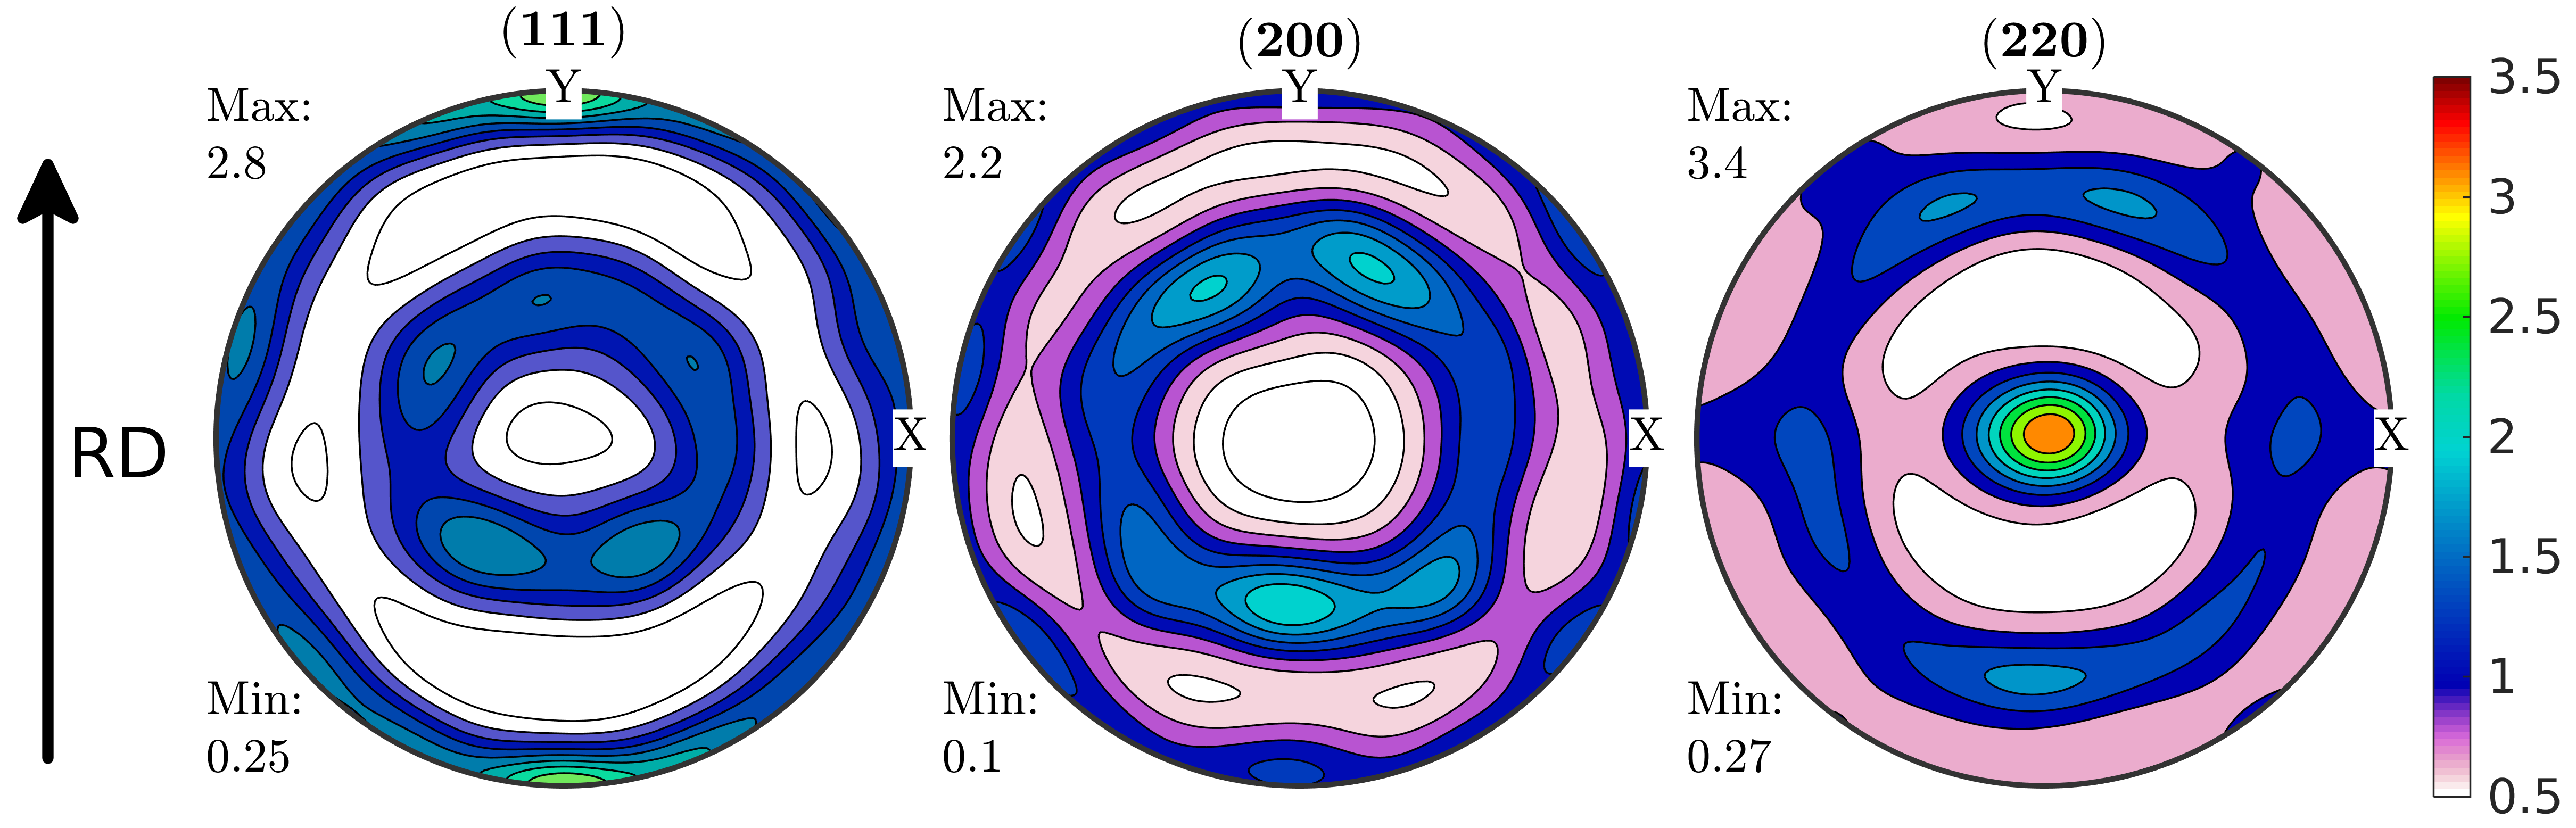
\includegraphics[width=\textwidth]{F138_Rec_RD}
  \caption{Textura F138 con sincrotron}
  \label{fig:F138PF}
\end{figure}


\begin{figure}[!htb]
  \centering
  \includegraphics[width=\textwidth]{F138_odf}
  \caption{ODF del F138}
  \label{fig:F138ODF}
\end{figure}


\newpage
\section{Estudio de la microestructura por el método de Langford y figuras de polos generalizadas}\label{S:F138LANG}
Al observar las FDO Generalizadas de Tamaño de cristalita y deformación, Figs. \ref{fig:F138Size} y \ref{fig:F138Strain} respectivamente, puede verse un comportamiento similiar al observado en el acero libre de intersticiales (Cap. \ref{C:IF}) en donde ciertas componentes favorecidas por la textura tienen mayor tamaño de cristalita y acumulan menos deformación, lo que en este caso se traduce a una menor densidad de dislocaciones.
En este caso puede verse que es la componente Goss es la componente que ``más limpia'', mientras que en la componente G/B(T) se tienen dominios un poco más grandes, pero con menor cantidad de dislocaciones acumuladas.
\begin{figure}[!htb]
  \centering
  \includegraphics[width=\textwidth]{F138_size_odf}
  \caption{Size ODF F138}
  \label{fig:F138Size}
\end{figure}

\begin{figure}[!htb]
  \centering
  \includegraphics[width=\textwidth]{F138_strain_odf}
  \caption{Strain ODF}
  \label{fig:F138Strain}
\end{figure}




\newpage
\section{Discusión de resultados}\label{S:F138Dis}
\newpage
\section{Conclusiones}\label{S:F138Conclusiones}

\chapter{Estudio sobre el acero duplex G2205}
\graphicspath{{./figs/06_G2205/}}
\section{Estudio de la microestructura por el método de Langford y figuras de polos generalizadas}\label{S:G2205LANG}
\section{Discusión de resultados}\label{S:G2205Dis}
\section{Conclusiones}\label{S:AlConclusiones}

\chapter{Estudio sobre el Aluminio 1050 laminado simétricamente}\label{C:AlS}
\graphicspath{{./figs/06_Al/}}

En este capítulo se estudiará la microestructura de chapas aluminio, laminadas simétricamente.
El aluminio es un material FCC con alta energía de falla de apilamiento y capacidad de recristalizar dinámicamente[ref].
Las chapas fueron obtenidas comercialmente y son de la aleación 1050, lo que significa que se trata de aluminio con baja cantidad de aleantes, y con capacidad de ser endurecido por trabajado.
Estas aleaciones poseen elevada ductilidad, resistencia a la corrosión y buena soldabilidad.\cite{ESAB:AlAlloys,AlOrg:AlAlloys,PAInt:AlAlloys}.
En estas condiciones se espera que el material sea fácil de deformar, lo que en el caso del laminado significa que se pueden lograr elevadas reducciones incluso deformando a temperatura ambiente.
Los usos principales de este material son aquellos en que la resistencia a la corrosión son importante, como ser la industria química y la alimenticia\cite{PAInt:AlAlloys,AZOM:AlAlloys}.
Debido a la tendencia de este material a recristalizar dinámicamente, también se espera que se acumulen pocas dislocaciones, ya que las mismas se pueden limpiar por recristalizado dinámico inducido por la deformación aplicada.

Los análisis realizados utilizando el método CMWP en las chapas estudiadas dan un valor promedio de factor de Wilkens del orden de la unidad, lo que indica que se puede suponer que existe poca correlación en las dislocaciones acumuladas, lo que a su vez hace a este material apropiado para ser estudiado dentro del modelo de Langford.
En particular, se estudiarán chapas de aluminio que desarrollaron texturas diferentes como producto del laminado: una que desarrolló la textura típica de laminado de los materiales con estructura cristalina FCC, y otra que mantuvo la textura cúbica de partida.

\section{Análisis de la textura}\label{S:AlText}
En la Fig. \ref{fig:AlPDF} se pueden observar las figuras de polos recalculadas para los dos aluminios laminados simétricamente, donde puede apreciarse claramente que ambos materiales han desarrollado texturas completamente diferentes.

Las chapas comerciales de aluminio provienen de un tren de laminado en caliente, lo que hace que estos materiales tengan como textura de partida la textura de recristalizado, que en el caso del aluminio puro es la textura cúbica[ref].

Los dos aluminios se laminaron de la misma manera, con la misma cantidad de pasos?

Sin embargo, la laminación simétrica con reducciones del 70\,\% o más suele introducir suficiente deformación en el material como para destruir completamente la textura de partida del mismo.
La textura de laminado del aluminio se caracteriza principalmente por componentes que se encuentran presentes a lo largo de la denominada fibra $\beta$, que va desde la orientación Cu = \{112\}\textless 111\textgreater, pasando por la orientación S = \{123\}\textless 634\textgreater, hasta la orientación Bs = \{011\}\textless 211\textgreater\cite{jata2013aluminum,Hirsch19882863,Engler1996187}.
La textura típica de los procesos de laminado simétrico en materiales FCC produce figuras de polos como la que se observa en la Fig.\,\ref{fig:AlPDF}-b, en cuyo caso se dice que el material tiene una textura de laminado de tipo cobre\cite{kocks2000texture}. Sin embargo, en materiales que tienden a recristalizar dinámicamente, si la textura cúbica de partida es muy intensa, puede ocurrir que la textura de recristalizado permanezca incluso a altas deformaciones, que es lo que ocurrió con la chapa cuyas FPs se ve en la Fig. \ref{fig:AlPDF}-a donde aparte de una intensa textura cúbica se puede apreciar una fibra \{001\}\textless 100\textgreater de baja intensidad.

\begin{figure}[!htb]
  \centering
  \includegraphics[width=0.8\textwidth]{AlText}
  \caption{Figuras de polos de dos chapas de aluminio 1050 laminadas hasta lograr una reducción del 70\,\%. En la Fig. (a) se puede apreciar que el aluminio conservó la textura cúbica de partida, mientras que en la (b) la chapa terminó adquiriendo la textura de laminado típica de un material FCC con alta energía de apilamiento.}
  \label{fig:AlPDF}
\end{figure}

La presencia de una textura cúbica o de laminado tipo cobre confirman la baja presencia de maclas y otro tipo de fallas de apilamiento en el material.
Como contraposición, el lector puede observar la textura de laminado del acero F138 en la Fig. \ref{fig:F138PF}, donde la presencia de aleantes ha bajado la energía de falla de apilamiento, lo que a su vez produce una textura de compresión con una fuerte presencia de la fibra \{110\}\textless 001\textgreater.
Cabe mencionar aquí también lo mencionado en el Cap. \ref{C:F138}, donde se mostró que la medición de la textura del acero F138 empleando rayos X de laboratorio mostró que el mismo exhibe la textura de laminado del latón, como era de esperarse.

En lo sucesivo, y para distinguir a ambos materiales, se denominará a la muestra que conservó la textura cúbica como $Al_C$, y a la muestra que desarrolló la textura de laminado como $Al_L$.

En la Fig. \ref{fig:AlODF} se pueden apreciar las secciones $\phi_2 \ = \ 0$\,$^{\circ}$ y $\phi_2 \ = \ 45$\,$^{\circ}$ de las muestras $Al_C$ (Fig. \ref{fig:AlODF}-a) y $Al_L$ (Fig. \ref{fig:AlODF}-b).

\begin{figure}[!htb]
  \centering
  \includegraphics[width=0.8\textwidth]{AlODF}
  \caption{FDO de las chapas de aluminio. Al observar las secciones $\phi_2 \ = \ 0$\,$^{\circ}$ y $\phi_2 \ = \ 45$\,$^{\circ}$ puede apreciarse más claramente que la principal componente de la textura de $Al_C$ es la cúbica, con una pequeña componente de fibra \{001\}\textless 100\textgreater, mientras que la muestra $Al_L$ tiene las componentes que se esperan en un material FCC laminado, es decir, la componente Goss y la \ldots}
  \label{fig:AlODF}
\end{figure}

\newpage
\section{Estudio de la microestructura de la muestra $Al_C$ por el método de Langford y figuras de polos generalizadas}\label{S:AlCLANG}

\begin{figure}[!htb]
  \centering
  \includegraphics[width=\textwidth]{FWHMvsODF_AlC}
  \caption{FWHM vs ODF para $Al_C$.}
  \label{fig:AlCFWHMODF}
\end{figure}

\begin{figure}[!htb]
  \centering
  \includegraphics[width=\textwidth]{MicrovsODF_AlC}
  \caption{Size y strain vs ODF $Al_C$.}
  \label{fig:AlCMicro}
\end{figure}

\newpage
\section{Estudio de la microestructura de la muestra $Al_L$ por el método de Langford y figuras de polos generalizadas}\label{S:AlLLANG}
\begin{figure}[!htb]
  \centering
  \includegraphics[width=\textwidth]{FWHMvsODF_AlL}
  \caption{FWHM vs ODF para $Al_L$.}
  \label{fig:AlLFWHMODF}
\end{figure}

\begin{figure}[!htb]
  \centering
  \includegraphics[width=\textwidth]{MicrovsODF_AlL}
  \caption{Size y strain vs ODF $Al_L$.}
  \label{fig:AlLMicro}
\end{figure}

\newpage
\section{Estudio de la microestructura por EBSD - Revisión}\label{S:AlEBSD}
\section{Discusión de resultados}\label{S:AlDis}
\section{Conclusiones}\label{S:AlConclusiones}

\chapter{Conclusiones}\label{C:Conclusiones}

\chapter{Proyecciones}\label{C:Proyecciones}


%\appendix
%\chapter{Archivos de entrada utilizados para correr los programas empleados en el desarrollo de esta tesis}\label{CA:input}
%\chapterquote{Negociemos Don Inodoro}{Fernando de la R\'{u}a, 2001}
%\chapterquote{Smartness runs in my family.  When I went to school I was so smart my teacher was in my class for five years}{George Burns}
\graphicspath{{figs/Apendice}}
En las secciones siguientes se muestran archivo de ejemplo de los archivos de entrada necesarios para la ejecución de los programas empleados en el transcurso de esta tesis.
El detalle acerca del flujo de trabajo puede encontrarse en el capítulo \ref{C:materiales}, y al final del nombre de cada archivo figura un número que indica el orden en que debe ingresarse cuando se corre el programa.
\section{Datos de entrada de IDEA}
\subsection*{Archivo \textit{data_info_1.ini}}
\begin{lstlisting}
1.PathForOutput     : /path/to/output/
2.NrOfSamples(1)    : 1

Input Data - 1
3.InputFilePath     : /path/to/spr/files/
4.InputFileName     : New_Al70R-tex_
5.FileExtension     : spr
6.IndexNr Start     : 1
7.Start Angle       : 1
8.IndexNr End       : 1
9.End Angle         : 1
10.DeltaIndexNr     : 1
11.Delta Angle      : 5
12.Start Gamma      : 0
13.End Gamma        : 359
14.Delta Gamma      : 5
15.Distance (mm)    : 1081
16.Pixel value (mm) : 0.1
17.Treshold         : 5
18.Printpattern(y/n): y
19.Correctwidth(y/n): y

Peak Positions
I. NrOfPeaks        : 7
II. Peak Positions
(2Theta Peak-L Peak-R BG-L BG-R):
1.742 583 713 400 935
2.013 713 854 500 965
2.850 1025 1130 965 1178
3.342 1215 1298 1190 1450
3.489 1298 1375 1190 1450
4.025 1505 1559 1450 1600
4.391 1650 1685 1620 1700
\end{lstlisting}


\subsection*{Archivo \textit{fit_ini_2.ini}}
\begin{lstlisting}
#FIT_INI: archivo con las estimaciones de los valores iniciales para el ajuste
#Peaks   Bg
7       19
#Global_H:
0.04500   
#Global_eta:
0.4400     
#2theta0    I0    shift_H    shift_eta
3.4840     2.0   0.0000     0.00000 
4.0240    64.0   0.0000     0.00000
5.6959    25.0   0.0000     0.00000
6.6794    17.0   0.0000     0.00000
6.9757     1.0   0.0000     0.00000
8.0569     6.0   0.0000     0.20000
8.7843     1.0   0.0000     0.50000
#Bg_pos(2theta) Bg_int
0.000       28.0050
0.360       28.0050
0.560       28.0050
0.880       28.0050
1.250       28.0050
2.050       44.8004
2.119       28.0050
2.648       28.0050
3.060       29.1600
4.369       34.2893
4.943       28.0050
5.048       25.1649
5.101       28.0050
6.219       28.0050
6.282       28.0050
7.640       28.0050
8.419       28.0050
8.523       28.0050
8.937       28.0050
\end{lstlisting}

\subsection*{Archivo \textit{IRF_3.dat}}

\subsection*{Conductividad térmica}
\begin{table}[h!]
  \centering
  \begin{tabular}{|c|c|}\hline
	Temperatura [K]	&	Conductividad térmica [W/(m K)]	\\ \hline
	7,500	&	1,260	\\
	13,750	&	3,900	\\
	20,000	&	6,803	\\
	25,625	&	9,639	\\
	32,500	&	12,411	\\
	36,875	&	14,193	\\
	40,000	&	14,855	\\
	41,250	&	15,515	\\
	46,250	&	16,377	\\
	50,000	&	17,566	\\
	55,625	&	18,626	\\
	61,250	&	19,554	\\
	67,500	&	20,352	\\
	73,750	&	21,084	\\
	78,750	&	21,485	\\
	84,375	&	21,887	\\
	91,875	&	22,358	\\
	100,000	&	22,763	\\
	106,875	&	22,772	\\
	110,625	&	23,172	\\
	118,750	&	23,183	\\
	134,375	&	23,203	\\
	149,375	&	23,157	\\
	159,375	&	23,236	\\
	174,375	&	23,453	\\
	185,625	&	23,600	\\
	194,375	&	23,677	\\
	204,375	&	23,690	\\
	216,250	&	23,969	\\
	230,625	&	24,382	\\
	247,500	&	24,602	\\
	260,625	&	25,146	\\
	277,500	&	25,826	\\
	292,500	&	26,174	\\ \hline
  \end{tabular}
  \caption[Tabla con los valores de la conductividad térmica del MgB$_2$.]{Tabla con los valores de la conductividad térmica del MgB$_2$. Datos obtenidos de \cite{Putti2003}.}
  \label{tab:kmgb2}
\end{table}
\newpage
\subsection*{Conductividad eléctrica}
La conductividad eléctrica del MgB$_2$ se obtuvo a partir de mediciones de resistividad obtenidas de \cite{Nagamatsu2001}. Como la conductividad eléctrica de un superconductor diverge para temperaturas que están por debajo de $T_c$, el estado superconductor se expresa por una conductividad eléctrica varios órdenes de magnitud mayor que la que tiene el material por encima de $T_c$.
\begin{table}[h!]
  \centering
  \begin{tabular}{|c|c|}\hline
	Temperatura [K]	&	Conductividad eléctrica [S/m]	\\ \hline
	4,710	&	100000000000,000	\\
	20,000	&	100000000000,000	\\
	34,960	&	100000000000,000	\\
	36,640	&	144034522,194	\\
	36,970	&	11074675,429	\\
	37,480	&	2486133,590	\\
	37,650	&	1728814,673	\\
	37,820	&	1414401,150	\\
	38,320	&	1363822,959	\\
	41,510	&	1354673,964	\\
	45,040	&	1354288,694	\\
	47,900	&	1349626,019	\\
	51,260	&	1349261,819	\\
	60,340	&	1339676,254	\\
	68,400	&	1330333,874	\\
	74,450	&	1325500,509	\\
	78,490	&	1325078,975	\\
	83,030	&	1316302,139	\\
	87,900	&	1307606,609	\\
	92,440	&	1299058,962	\\
	96,970	&	1294600,609	\\
	99,500	&	1290372,531	\\ \hline
  \end{tabular}
  \caption[Tabla con los valores de la conductividad eléctrica del del MgB$_2$.]{Tabla con los valores de la conductividad eléctrica del del MgB$_2$. Datos obtenidos de \cite{Nagamatsu2001}.}
  \label{tab:smgb2}
\end{table}
\newpage
\section{Propiedades físicas del silicio}
\subsection*{Calor específico}
Como se explicó al principio del capítulo, los valores de calor específico del silicio no se obtuvieron de tablas, sino de las librerías de propiedades físicas del programa COMSOL MULTIPHYSICS. Este programa utiliza polinomios para aproximar los valores de calor específico. El polinomio que utiliza es de la forma $p_0(T) \,=\, A_0\,+\,A_1 \times T\,+\,A_2 \times T^2\,+\,A_3 \times T^3\,+\,A_4 \times T^4\,$, y los coeficientes del polinomio dependen del intervalo de temperatura considerado. En la tabla \ref{tab:csi} se muestran los coeficientes de dicho polinomio para cada intervalo de temperatura.
\begin{table}[h!]
  %\centering
  \hspace{-1.6cm}
  \begin{tabular}{|c|c|c|c|c|c|c|}\hline
$T_{i}\,[\rm K]$	&	$T_{f}\,[\rm K]$	&	$A_0\,[\rm J/(\rm Kg\,K)]$	&	$A_1\,[\rm J/(\rm Kg\,K^2)]$	&	$A_2\,[\rm J/(\rm Kg\,K^3)]$	&	$A_3\,[\rm J/(\rm Kg\,K^4)]$	&	$A_4\,[\rm J/(\rm Kg\,K^5)]$	\\ \hline
1.0	&	7.0	&$	-4.83\,10^{-5}	$&$	7.68\,10^{-5}	$&$	-3.42\,10^{-5}	$&$	2.81\,10^{-4}	$&$	-3.13\,10^{-7}	$\\ \hline
7.0	&	20.0	&$	0.0525	$&$	-0.0396	$&$	0.0100	$&$	-7.81\,10^{-4}	$&$	3.96\,10^{-5}	$\\ \hline
20.0	&	50.0	&$	-1.81	$&$	0.762	$&$	-0.0865	$&$	0.00374	$&$	-3.33\,10^{-5}	$\\ \hline
50.0	&	293.0	&$	-82.9	$&$	2.71	$&$	0.0140	$&$	-7.98\,10^{-5}	$&$	1.08\,10^{-7}	$\\ \hline
293.0	&	900.0	&$	63.0	$&$	3.77	$&$	-0.00695	$&$	5.95\,10^{-6}	$&$	-1.91\,10^{-9}	$\\ \hline
900.0	&	1685.0	&$	769.0	$&$	0.187	$&$	-3.18\,10^{-5}	$&$	0	$&$	0	$\\ \hline
  \end{tabular}
  \caption[Tabla con coeficientes del polinomio utilizado para calcular el calor específico del silicio.]{Tabla con coeficientes del polinomio utilizado para calcular el calor específico del silicio. El polinomio propuesto es de la forma $p_0(T) \,=\, A_0\,+\,A_1 \times T\,+\,A_2 \times T^2\,+\,A_3 \times T^3\,+\,A_4 \times T^4$. Datos obtenidos de la biblioteca de materiales del programa COMSOL MULTIPHYSICS.}
  \label{tab:csi}
\end{table}
\newpage
\subsection*{Conductividad térmica}
\begin{table}[h!]
  \centering
  \begin{tabular}{|c|c|}\hline
	Temperatura [K]	&	Conductividad térmica [$\frac{\rm W}{\rm m\ K}$]	\\ \hline
	6,897	&	0,0264	\\
	8,513	&	0,0481	\\
	10,251	&	0,0765	\\
	13,628	&	0,1292	\\
	16,821	&	0,1868	\\
	19,039	&	0,2226	\\
	21,548	&	0,2602	\\
	23,792	&	0,2926	\\
	26,928	&	0,3229	\\
	30,478	&	0,3495	\\
	35,801	&	0,3715	\\
	41,024	&	0,3655	\\
	52,553	&	0,3338	\\
	62,500	&	0,2873	\\
	75,256	&	0,2291	\\
	88,400	&	0,1724	\\
	101,299	&	0,1373	\\
	116,080	&	0,1033	\\
	158,197	&	0,0541	\\
	221,000	&	0,0289	\\
	316,476	&	0,0164	\\
	415,574	&	0,0115	\\ \hline
  \end{tabular}
  \caption[Tabla con los valores de la conductividad térmica del silicio.]{Tabla con los valores de la conductividad térmica del silicio. Datos obtenidos de \cite{Glassbrenner1964}.}
  \label{tab:ksi}
\end{table}
\newpage
\section{Propiedades físicas del zafiro}
Al igual que para el caso del calor específico del silicio, el calor específico y la  conductividad térmica del zafiro se obtuvieron a partir de polinomios en $T$, y en las tablas subsiguientes se muestran los coeficientes de dichos polinomios. El calor específico se obtuvo a partir de un polinomio del tipo $p_1(T) \,=\, A_0\,+\,A_1 \times T\,+\,A_2 \times T^2\,+\,A_3 \times T^3\,+\,A_4 \times T^4$, mientras que la conductividad térmica se calculó de un polinomio de grado 5, es decir que $\kappa_{\rm zafiro} \ \approx \ p_2(T) \,=\, A_0\,+\,A_1 \times T\,+\,A_2 \times T^2\,+\,A_3 \times T^3\,+\,A_4 \times T^4\,+\,A_5 \times T^5$.
\subsection*{Calor específico}
\begin{table}[h!]
  %\centering
  \hspace{-1.6cm}
  \begin{tabular}{|c|c|c|c|c|c|c|}\hline
$T_{i}\,[\rm K]$	&	$T_{f}\,[\rm K]$	&	$A_0\,[\rm J/(\rm Kg\,K)]$	&	$A_1\,[\rm J/(\rm Kg\,K^2)]$	&	$A_2\,[\rm J/(\rm Kg\,K^3)]$	&	$A_3\,[\rm J/(\rm Kg\,K^4)]$	&	$A_4\,[\rm J/(\rm Kg\,K^5)]$	\\ \hline
10.0	&	60.0	&$	-0.392	$&$	0.0802	$&$	-0.00507	$&$	1.91\,10^{-4}	$&$	1.78\,10^{-17}	$\\ \hline
60.0	&	130.0	&$	30.0	$&$	-1.46	$&$	0.0191	$&$	1.12\,10^{-4}	$&$	-6.09\,10^{-7}	$\\ \hline
130.0	&	300.0	&$	-42.6	$&$	-1.40	$&$	0.0434	$&$	-1.45E\,10^{-4}	$&$	1.55\,10^{-7}	$\\ \hline
300.0	&	810.0	&$	-528	$&$	7.53	$&$	-0.0139	$&$	1.243\,10^{-5}	$&$	-4.33\,10^{-9}	$\\ \hline
810.0	&	2250.0	&$	745	$&$	0.956	$&$	-7.12\,10^{-4}	$&$	2.69\,10^{-7}	$&$	-3.85\,10^{-11}	$\\ \hline
  \end{tabular}
  \caption[Tabla con coeficientes del polinomio utilizado para calcular el calor específico del zafiro.]{Tabla con coeficientes del polinomio utilizado para calcular el calor específico del zafiro. El polinomio propuesto es de la forma $p_1(T) \,=\, A_0\,+\,A_1 \times T\,+\,A_2 \times T^2\,+\,A_3 \times T^3\,+\,A_4 \times T^4$. Datos obtenidos de la biblioteca de materiales del programa COMSOL MULTIPHYSICS.}
  \label{tab:czaf}
\end{table}

\subsection*{Conductividad térmica}
\begin{table}[h!]
  \centering
  %\hspace{-1.6cm}
  \begin{tabular}{|c|c|c|c|c|}\hline
$T_{i}\,[\rm K]$	&	$T_{f}\,[\rm K]$	&	$A_0\,[\rm J/(\rm Kg\,K)]$	&	$A_1\,[\rm J/(\rm Kg\,K^2)]$	&	$A_2\,[\rm J/(\rm Kg\,K^3)]$	\\ \hline
6.0	&	47.0	&$	-5.11	$&$	1.76	$&$	-0.167	$\\ \hline
47.0	&	108.0	&$	-422	$&$	24.9	$&$	-0.385	$ \\ \hline
108.0	&	300.0	&$	316	$&$	-2.90	$&$	0.0125	$\\ \hline
300.0	&	2073.0	&$	75.8	$&$	-0.190	$&$	2.02\,10^{-4}	$\\ \hline
-&-&-&-&-\\ \hline	
$T_{i}\,[\rm K]$	&	$T_{f}\,[\rm K]$	&	$A_3\,[\rm J/(\rm Kg\,K^4)]$	&	$A_4\,[\rm J/(\rm Kg\,K^5)]$	&	$A_5\,[\rm J/(\rm Kg\,K^6)]$ \\ \hline
6.0	&	47.0	&$	0.0127	$&$	-2.59\,10^{-4}	$&$	1.64\,10^{-6} $\\ \hline
47.0	&	108.0	&$	0.00268	$&$	-8.82\,10^{-6}	$&$	1.12\,10^{-8}	$\\ \hline
108.0	&	300.0	&$	-2.77\,10^{-5}	$&$	3.10\,10^{-8}	$&$	1.37\,10^{-11}	$\\ \hline
300.0	&	2073.0	&$	-9.79\,10^{-8}	$&$	1.78\,10^{-11}	$&$	0	$\\ \hline
  \end{tabular}
  \caption[Tabla con coeficientes del polinomio utilizado para calcular la conductividad térmica del zafiro.]{Tabla con coeficientes del polinomio utilizado para calcular la conductividad térmica del zafiro. El polinomio propuesto es de la forma $p_2(T) \,=\, A_0\,+\,A_1 \times T\,+\,A_2 \times T^2\,+\,A_3 \times T^3\,+\,A_4 \times T^4\,+\,A_5 \times T^5$. Datos obtenidos de la biblioteca de materiales del programa COMSOL MULTIPHYSICS.}
  \label{tab:kzaf}
\end{table}
%%%%%%%%%%%%%%%%%%%%%%%%%%%%%%%%%%%%%%%%%%%%%%%%%%%%%%%%%%%%%%%%%%%%%%%%


\begin{biblio}
  \bibliography{./bib/library,./bib/Physical_Properties_of_Crystals.bib,./bib/International_Tables_for_Crystallography.bib}
\end{biblio}

\begin{postliminary}

%\begin{seccion}{Publicaciones asociadas}
%  \begin{enumerate}
%  \item Mi primer aviso en la revista \textbf{ABC}, 1996
%  \item Mi segunda publicaci\'{o}n en la revista \textbf{ABC}, 1997
%  \end{enumerate}
%\end{seccion}

\end{postliminary}

\end{document}
